%pdflatex -shell-escape *.tex
\documentclass{standalone}
\usepackage{amsmath,amsfonts,amssymb}
%
\usepackage{graphicx}
\graphicspath{ {images/} }
%
\usepackage{xcolor}
\pagestyle{empty}
\pagecolor{white}
%
\everymath{\displaystyle}
%
\usepackage{CJKutf8}   %CJKspace
\AtBeginDvi{\input{zhwinfonts}}
%%%
\newcommand{\zh}[1]{\begin{CJK*}{UTF8}{zhsong}#1\end{CJK*}}
\newcommand{\YBao}{\color{red}\zh{源宝爱数学}}
\newcommand{\BT}[1]{\color{red}\zh{#1}\color{black}}
\newcommand{\fTxT}[1]{\text{\zh{#1}}}
%

\immediate\write18{pdflatex test.tex}
\immediate\write18{convert -density 150 -adaptive-resize 480x480 test.pdf test.jpg}
%
\usepackage{tikz}
%\usetikzlibrary{intersections} 
%\usetikzlibrary{calc,fadings,decorations.pathreplacing} 
\usetikzlibrary{math}
\usepackage{ifthen}
\newcounter{count}
% 
%
\begin{document}
\begin{minipage}[b][14cm][t]{1.00\textwidth}
%
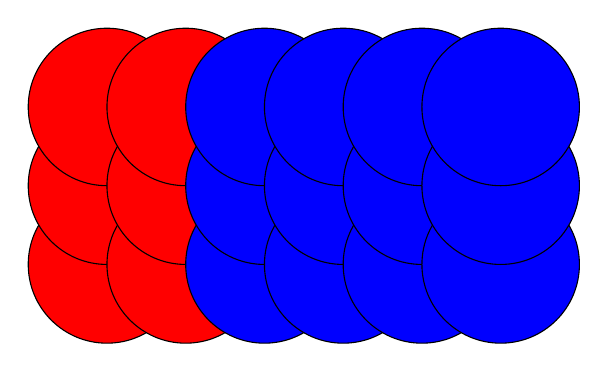
\begin{tikzpicture} 
  \def\clr{red}% initial color
  \setcounter{count}{0}% initial counter 
  \foreach \col in {1,...,6}
  {
    \foreach \row in {1,...,3}
       {
         \stepcounter{count}
         \ifthenelse{\value{count}>6}{\def\clr{blue}}{}
         \draw[fill=\clr] (\col,\row) ellipse (1cm and 1cm);
       }
  }
\end{tikzpicture}
% 
\end{minipage}\end{document}
% \begin{tikzpicture} 
% \coordinate (O) at (0,0); 
% \coordinate (A) at (2.0,2.0); 
% \draw [name path = c1, red, thick] (A) circle [radius = 4cm]; 
% \draw [name path = c2, green, thin] (A) ellipse (5.0cm and 2.0cm); 
% \draw [execute at begin node={\global\let\t=\t},
%        name intersections = {of = c1 and c2,total=\t}] 
% (intersection-1) -- (intersection-2) -- (intersection-3) 
% -- (intersection-4) -- cycle; 
% \pgfmathsetmacro{\nr}{0}
% \foreach \point in {1,...,\t}
%   \filldraw[red] (intersection-\point) circle (0.5cm);
% \end{tikzpicture} 
